\chapter{Rękawice jako kontrolery}
\label{ch:kontrolery}
Kontroler w postaci rękawicy jest pojęciem często używanym ze względu na popularność tego rozwiązania. Rękawiczka zakładana na dłoń z zamontowanymi czujnikami dzięki którym deweloper uzyskuje wszelkie potrzebne informacja aby wchodzić w interakcję z otoczeniem. Idea która za tym stoi nie dotyczy jednak rękawiczki samej w sobie - chodzi o wykorzystanie ludzkiej dłoni jako kontrolera a rękawiczka jest używana jako nośnik temu służący. Ze względu na różne podejścia istnieją typy kontrolerów wykorzystujących dłoń do obsługi świata, które zostaną opisane w dalszej części tego rozdziału. Kontrolery a w szczególności dłonie są głównie wykorzystywane w świecie VR, w pozostałych rodzajach XR wystarczyłaby analiza obrazu na podstawie której określa się interakcję użytkownika z otoczeniem. W przypadku VR które przenosi użytkownika do zupełnie innego świata, wykorzystanie kontrolerów wydaję się więc obowiązkowe.  
\section{Rozwój rękawicy jako kontrolera}
\label{sec:rozwojVR}
	Pomysł wykorzystania dłoni jako kontrolera, pomimo wielu lat od pierwszego wdrożenia wciąż znajduje zastosowania głównie w biznesie, jednak produkty te są dostępne również dla zwykłych konsumentów. Problemem jest jednak cena która czasami wynosi tyle co zestaw do obsługi VR bądź więcej. Oprócz tego nie ma zbyt wielu pozycji w sklepie które by wykorzystywały w sposób szczególny tego rodzaju kontrolery. Dlatego też to właśnie głownie firmy są zainteresowane tego typu produktami, które dla specyficznego przypadku tworzą aplikacje obsługujące tego typu kontrolery. Wykorzystanie XR i rękawic kontrolerów w biznesie pokazano w rozdziale~\ref{ch:biznes}. Jednak aby produkt ten był w stanie spełnić oczekiwania rynku musiał przejść długą drogę od projektu stworzonego przez Dana Sandina. Jego rękawica \textit{The Sayre Glove} była w pełni przewodowa a jedynymi czujnikami które obsługiwała był pomiar wygięcia palców, służący głównie do zmiany pozycji suwaków. Była jednak tania i lekka co spełniało podstawowe oczekiwania w tamtych czasach. Rękawice tą przedstawia rysunek~\ref{fig:sayra}.
\begin{figure}[h]
\centering
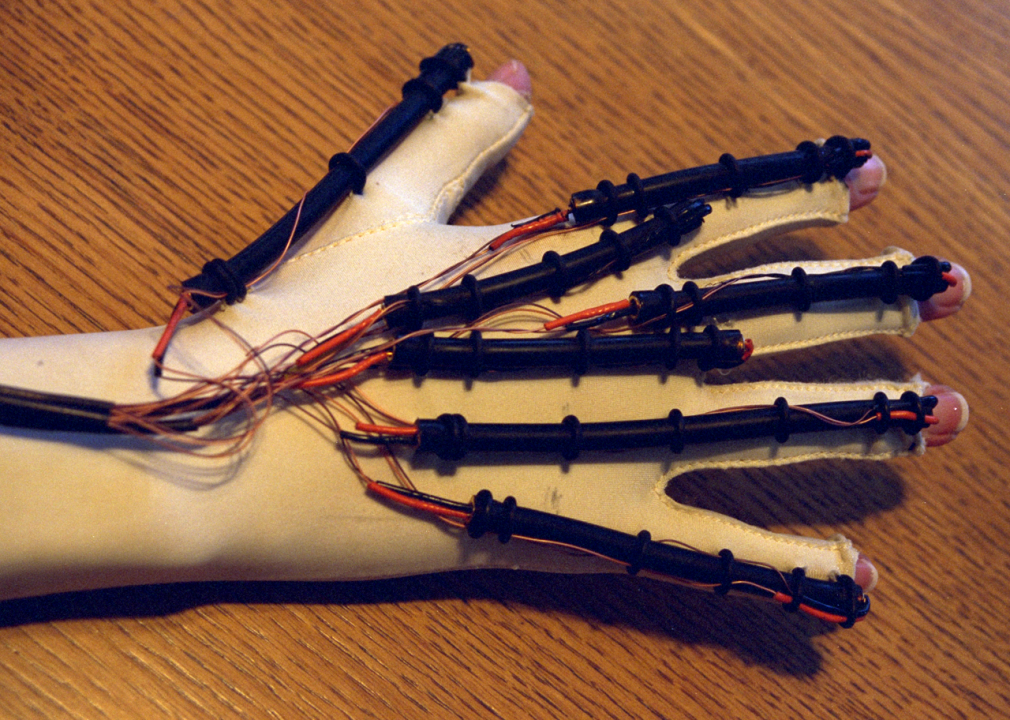
\includegraphics[width = 0.7\textwidth]{sayra}
\captionsource{Pierwsza rękawica VR - Sayra Glove}{\url{https://www.evl.uic.edu/entry.php?id=2162}}
\label{fig:sayra}
\end{figure}
W 1983 roku Gary Grimes stworzył kolejny produkt warty uwagi - była to rękawica która potrafiła rozpoznawać osiemdziesiąt specjalnych gestów, które następnie były zamieniane na litery alfabetu. Produkt ten jednak nie został nigdy dostępny do kupienia. Kilka lat później, w 1987 roku nastąpił przełom w dziedzinie rękawic kontrolerów. Została stworzona rękawica która potrafiła monitorować sześć stopni swobody - oznacza to przemieszczenie oraz orientację wokół trójwymiarowego układu współrzędnych. Wykonana została przez Thomasa Zimmermana wraz ze współpracownikami i została spopularyzowana i rozpowszechniona na całym świecie. Niewątpliwie był to największy przeskok w rozwoju tego urządzenia od czasu pierwszego projektu. Dwa lata później powstała rękawica która jako pierwsza była dostępna w celach rozrywkowych. Stworzona przez firmę zabawkową Mattel, dla gier konsolowych produkowanych przez Nintendo, rękawica nazwana \textit{The Power Glove}. Produkcja jednak została przerwana po dwóch latach od wprowadzenia na rynek produktu. Są to wybrane pozycje które w jakimś stopniu zmieniły rynek oraz wprowadziły zmiany w tym segmencie. Wraz z dalszym rozwojem wirtualnej rzeczywistości powstały kolejne produkty a w szczególności po roku 2000, podczas pierwszej fali popularności technologii VR powstało wiele dopracowanych produktów~\cite{ewolucja}. 
\section{Podział rękawic-kontrolerów}
\label{sec:podzial}
Rozwój rękawic-kontrolerów wprowadził wiele zmian począwszy od technologii na której bazują, połączeń które używają jak i funkcjonalności które są w stanie zapewnić. Na tej podstawie nadal większość produktów stara się wyróżnić na tle konkurencji jednak bazowe podejście do produktu sprawia że można go podzielić według ogólnych kategorii, do których można zaliczyć rękawice klasyczne, systemy nasadowe oraz egzoszkielety. W dalszych częściach tej sekcji zostaną opisane szczegółowo te typy wraz z prezentacją współczesnych rozwiązań które są dostępne na rynku~\cite{review}. 

	\subsection{Klasyczne}
	\label{subsec:klasyczne}
	Pierwsze, najstarsze typy rękawic określane są jako klasyczne ponieważ przypominają one zwykłe rękawiczki używane w życiu codziennym z tym że podpięto do nich różnego rodzaju sensory, mikrokontrolery, przekaźniki danych i baterie. Innymi słowy sprawiono że zwykła rękawiczka jest w stanie zbierać dane na temat położenia dłoni i palców użytkownika, a następnie bezprzewodowo przesłać te dane do odbiornika, zapewniając przy tym wygodę pracy oraz ponad kilka godzin użytkowania na jednym ładowaniu w zależności od produktu. Prawdopodobnie najbardziej znanym produktem na rynku są rękawice należące do firmy Manus Vr, która dostarcza kilka rozwiązań w zależności od dodatku za które użytkownik chce dopłacić. Wykonane z elastycznego materiału, lekkie i cienkie dzięki czemu są przyjemne w używaniu, z materiałem odciętym w czubkach palców dla większej wygody. Waga to około 70 gramów, co sprawia że użytkowanie to czysta przyjemność. Rękawice łączą się z takimi zestawami VR jak Oculus czy Vive i są szeroko wykorzystywane na rynku biznesowym przez takie firmy jak Audi, BMW, Ubisoft czy NASA. Cena za rękawice to od 3000 do 4000 euro - zdecydowanie nie należą one do najtańszych. Od strony technicznej, w początkowej wersji tego projektu zostały zastosowane czujniki oporu, które zwracały różny opór, jednak zastąpiono je w nowszej wersji zestawem  czujników zaprojektowane przez firmę Bosch w skład których wchodzą jedenaście czujników na palcach, dwa na każdym poza kciukiem gdzie znajdują się trzy - żyroskop, akcelerometr i magnetometr dla dokładnego mierzenia położenia naszej dłoni. Czujniki te są elastyczne i działają analogowo sprawdzając knykcie oraz pierwszy staw palca a także od knykci do drugiego stawu palca łącznie dając dziesięć stref pomiaru. Czujniki orientacyjne znajdują się na wierzchniej części dłoni oraz kciuka - pomiar jest dokonywany dzięki płytce IMU zapewniającej jedenaście stopni swobody. Czujniki na palcach wskazują dokładność $\pm 3$ stopni. System śledzenia natomiast oblicza pozycję dłoni w przestrzeni dzięki użyciu innych systemów takich jak Xsens, Vive Tracking, OptiTrack, Vicon czy ART. Obsługują one pracę wielu użytkowników jednocześnie w jednym świecie wirtualnym. Bateria została wyprodukowana przez firmę Varta a producent szacuję czas pracy na baterii pomiędzy 4 a 6 godzinami intensywnego użytkowania. Rękawice działają bezprzewodowo przy opóźnieniu poniżej 5 milisekund. Wspierają one również technologię wibracji, dzięki czemu można samodzielnie zaprogramować moduł wibrujący dla odpowiednich czynności świata wirtualnego. Firma wypuściła własne wtyczki dla takich środowisk jak Unity, Unreal Engine oraz Autodesk MotionBuilder. Jest to jedno z najbardziej rozbudowanych rozwiązań na rynku które wspiera rozwój swojego oprogramowania na wielu platformach i stanowi jednego z największych konkurentów dla pozostałych produktów~\cite{manus}. Rękawice te widoczne są na rysunku~\ref{fig:manus}. Podobnym produktem występującym na rynku są rękawice firmy Noitom o nazwie \textit{Hi5}. Rękawice te kosztują znacznie mniej, ich cena to około 1000\$, jednak posiadają znacznie wiecej wad. Przede wszystkim nie wspierają one zestawu Oculus Rift. Tak jak w poprzednim przypadku, bazują one na kontrolerach ruchu dostarczonych przez zewnętrzną firmę - w tym przypadku są to kontrolery Vive. Źródłem zasilania są zwykłe baterie AA co stanowi poważny problem dla dłuższego użytkowania. Rękawice wspierają \textit{Haptic Feedback}, czyli system wibracji oparty na interakcji z przedmiotami w świecie wirtualnym, zapewniają śledzenie wszystkich palców u dłoni oraz używają czujników takich jak żyroskop, akcelerometr i magnetometr wbudowanych w jednostkę IMU. Widać więc że spełniają one stawiane przed tymi kontrolerami oczekiwania jednak posiada wiele niedociągnięć które potencjalnie zniechęcają do kupna tego produktu~\cite{hi5}. Rysunek~\ref{fig:hi5} przedstawia omawiany kontroler.
\begin{figure}[h]
\centering
	\begin{subfigure}[b]{0.4\textwidth}
	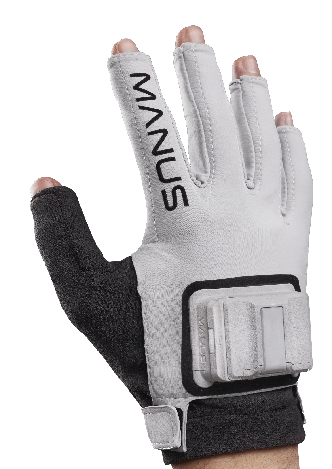
\includegraphics[width=\textwidth]{manus}
	\captionsource{Rękawica firmy Manus Vr}{\url{https://manus-vr.com/mocapgloves}\\}
	\label{fig:manus}
	\end{subfigure}
	\hspace{0.5cm}
	\begin{subfigure}[b]{0.34\textwidth}
	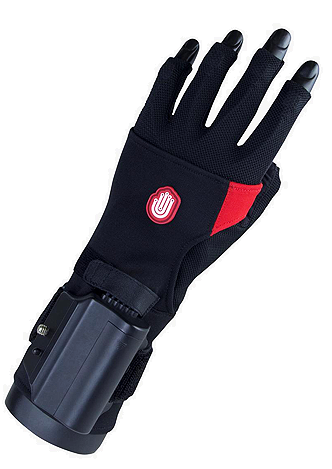
\includegraphics[width=\textwidth]{hi5}
	\captionsource{Rękawica firmy Noitom}{\url{https://hi5vrglove.com/store/hi5glove}}
	\label{fig:hi5}
	\end{subfigure}
\caption{Przykładowe klasyczne rękawice VR.}
\label{fig:rekawice}
\end{figure}	
Kolejnym produktem jest \textit{Exoglobe}, który wyróżnia się na tle konkurencji dzięki zastosowania technologii ultradźwięków. W ten sposób śledzi dłoń w prawie $180^o$ z dokładnością nawet do 0,5 mm. W oprogramowaniu rękawic znajduję się moduł sztucznej inteligencji który uczy się gestów, sposobu poruszania się oraz obszaru w którym porusza się użytkownik. Wszystko zapewniane jest za cenę 99\$ która jest zdecydowanie mniejsza od propozycji konkurencji~\cite{exo}. Avatar VR jest to produkt hiszpańskiej firmy NeuroDigital, która stworzyła rękawicę wspierającą haptic feedback, wykonaną z oddychającego materiału który również jest materiałem przewodzącym co pozwoliło zaimplementować sterowanie gestami. Za cenę 1500\$ dostajemy parę rękawiczek wraz z odbiornikiem USB który łączy się poprzez Bluetooth 4.0. Produkt zapewnia od sześciu do ośmiu godzin pracy na baterii po której należy naładować akumulator poprzez 5 V micro USB. Do rękawiczek można podłączyć odpowiednie czujniki które należy podpiąć na ramieniu oraz klatce co zapewnia śledzenie całej górnej części ciała. Sterowanie zapewniane jest poprzez 9 osiowe IMU. Rękawiczki mają wbudowanych 10 płytek wibrujących które zapewniają 1024 różnych poziomów wibracji. W rękawiczkach znajdują się 4 strefy przewodzące (dłoń, kciuk, palec wskazujący oraz środkowy). Produkt posiada również technologię NZDE (z ang. Near zero drift Experience), która pozwala powtarzać te same gesty w celu eksperymentowania w środowisku wirtualnym bez wprowadzania kumulacji znaczących błędów które gromadzą się w szczególności przy korzystaniu z danych żyroskopu~\cite{avatar}. Ostatnim produktem z kategorii klasycznych rękawic który warto wymienić są rękawice CaptoGlove. Firma produkująca ten kontroler rozszerza swoją funkcjonalność poza świat VR. Producent daje możliwość używania swoich rękawic poprzez technologię plug and play (z ang. podłącz i używaj) z komputerami oraz smart-fonami. Dzięki użyciu zapewnianego sdk można dalej przenieść nasze doświadczenia na platformy VR, konsole do gier czy kontrolować przy ich użyciu drony, roboty czy telewizory. Za pojedynczą rękawice klient zapłaci 250\$ za parę natomiast 490\$. Aby używać produktu w VR, grach wideo czy na smart urządzeniach należy dokupić Capto sensor czyli czujnik ruchu pozwalający określić położenie dłoni w przestrzeni kosztujący dodatkowe 190\$. Urządzenia kontrolujemy przy użyciu gestów dłoni, odpowiednie ruchy są tłumaczone na akcji wykonywane na różnych platformach. Na czubkach palców został umieszczony materiał pozwalający kontrolować ekrany dotykowe bez zdejmowania kontrolera. Rękawica łączy się z wymienionymi urządzeniami przy pomocy Bluetooth i według producenta pozwala na pracę przez około 10 godzin. Jest to kolejna pozycja wśród rękawic ciesząca się popularnością i jest wykorzystywana przez takie firmy i organizacje jak Mitsubishi, U.S. Air Force czy Fujitsu~\cite{capto}.  
	
	\subsection{Nasadowe}
	\label{subsec:nasadowe}
	Kolejnym typem urządzeń pozwalających na używanie dłoni jako kontrolera są urządzenia nasadowe. Nie są to typowe rękawiczki, a jedynie jej elementy których można by się spodziewać na czubkach palców, nadgarstkach czy też dłoni, które połączone odpowiednio ze sobą pozwalają na odczytywanie danych dotyczących położenia i orientacji  dłoni, palców, zapewniają wibracją oraz innego rodzaju imitacje świata rzeczywistego. W tym segmencie zdecydowanie wyróżniają się nakładki na palce, które skupiają się na symulacji dotyku, a w szczególności dwie firmy które się tym zajmują - Tactai z nakładką na palec nazwaną Tactai Haptic Module oraz GoTouchVR ze swoim produktem VrTouch. Pierwsza z tych firm zajmuje się stworzeniem małego urządzenia zakładanego na czubki palców które pozwala poczuć świat wirtualny. Firma ta zajmuje się badaniem tego jak ludzie odczuwają różne przedmioty w świecie rzeczywistym poprzez zmysł dotyku i stara się imitować te same odczucia dla zdarzeń zachodzących w świecie wirtualnym. Poprzez specjalne urządzenie przypominające długopis, rejestruje wibracje różnych materiałów i ich teksturę, następnie tworzy w systemie wzory wibracji, dokładając do tego dźwięki, jakie wspomniane materiały wydają podczas poruszania po nich urządzeniem badawczym. Następnie na podstawie zebranych danych, imitująto samo zjawisko gdy użytkownik wchodzi w interakcje z danym materiałem  w świecie wirtualnym. Oprócz tego znajduję się tam również mechanizm pozwalający na śledzenie palca. Konstrukcja ta pokazana jest na rysunku~\ref{fig:tactai}~\cite{tactai}. Druga firma obrała inny kierunek przy tworzeniu produkty, ich nakładki na palce są rozszerzeniem które można wykorzystać z już istniejącymi produktami rękawiczek, dzięki czemu można wykorzystać wbudowane w nie systemy śledzenia. Firma ta współpracuje z urządzeniami firm takich jak Manus czy Noitom. Ich urządzenia współpracuje z trzema nakładkami jednocześnie dla każdej z dłoni przy zapewnieniu niskiego poziomu opóźnienia. Poza tym ich funkcjonalność jest taka sama jak prezentowanej w tej sekcji konkurencji - pod względem wyglądu natomiast urządzenia ta przypominają nie wyglądają zbyt nowocześnie. GoTouchVr współpracuje głównie w ramach sektora biznesowego i medycznego dostarczając swoich rozwiązań do takich firm jak BMW czy Medtronic. Urządzenie to pokazane jest na rysunku~\ref{fig:touchVr}~\cite{touchVr}.

\begin{figure}[h]
\centering
	\begin{subfigure}[b]{0.4\textwidth}
	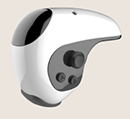
\includegraphics[width=\textwidth]{tactai}
	\captionsource{Urządzenie Tactai}{\url{https://www.tactai.com/company}\\}
	\label{fig:tactai}
	\end{subfigure}
	\hspace{0.5cm}
	\begin{subfigure}[b]{0.4\textwidth}
	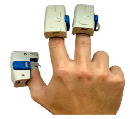
\includegraphics[width=\textwidth]{touchVr}
	\captionsource{Urządzenie TouchVr}{\url{https://www.gotouchvr.com/copy-of-technology-devices-1}}
	\label{fig:touchVr}
	\end{subfigure}
\caption{Urządzenia nasadowe.}
\label{fig:tactails}
\end{figure}

	\subsection{Egzoszkielety}
	\label{subsec:egzo}	
	Ostatnim rodzajem kontrolerów które bazują na ruchu dłoni i zarazem tych które podejmują niejako największe wyzwanie są egzoszkielety. Rękawica typu egzoszkielet, jak sama nazwa wskazuje, jest to rodzaj rękawicy posiadający swojego rodzaju szkielet zewnętrzny. Szkielet ten przymocowany wokół rąk użytkownika służy jako dodatkowa blokada dłoni, dzięki czemu użytkownik świata wirtualnego otrzymuje te same odczucia oporu wynikające z przedmiotów jak w świecie rzeczywistym. Gdy w świecie wirtualnym użytkownik takiego szkieletu ściska kamień, jego dłoń jest blokowana w odpowiednich miejscach, w zależności od danych uzyskanych ze świata wirtualnego który definiuje to jaką pozycję ręka użytkownika może maksymalnie przyjąć. Jest to rodzaj kontrolera nasadowego który pozwala poczuć świat wirtualny jednak nie w dosłownym tego znaczeniu. Uzyskane w ten sposób uczucia nie imitują dotyku przedmiotu a jedynie symulują opór jaki te przedmioty wytwarzają. Ludzki mózg jednak zawsze stara znaleźć się wyjaśnienie dla danego zjawiska, w związku z tym samoistnie łączy bodźce wzrokowe z blokadą motoryczną ręki, nadając tym samym generowanym komputerowo przedmiotom wyższy realizm. Istnieje wiele firm zajmujących się tego typu projektami jednak w tym rozdziale zostanie opisane tylko kilka których w sposób szczególny wyróżniają się na tle konkurencji.
	 Projekt taki stworzyła chińska firma Dexta Robotics, która wystartowała z kampanią finansowania społecznego w 2014 roku, jednak zbiórka pieniędzy zakończyła się niepowodzeniem. Była to jedna z pierwszych  spopularyzowanych rękawic egzoszkieletów, która pomimo porażki w zbiórce pieniędzy przetrwała i firma dokończyła projekt na własną rękę w 2016 roku. Egzoszkielet ten pozwala zatrzymać rękę gdy trafi na odpowiedni obiekt a także stopniowo aplikować opór gdy jest ściskany obiekt który ten opór zmienia w zależności od poziomu nacisku. Minusem tego rozwiązania jest opór który zostaje nakładany jedynie na czubki palców, co sprawia że traci się w pewnym stopniu realizm interakcji. Sam wygląd rękawicy jest natomiast bardzo futurystyczny - rękawica przedstawiona jest na rysunku~\ref{fig:dexmo}~\cite{dexta}.
	 \begin{figure}[h]
	 \centering
	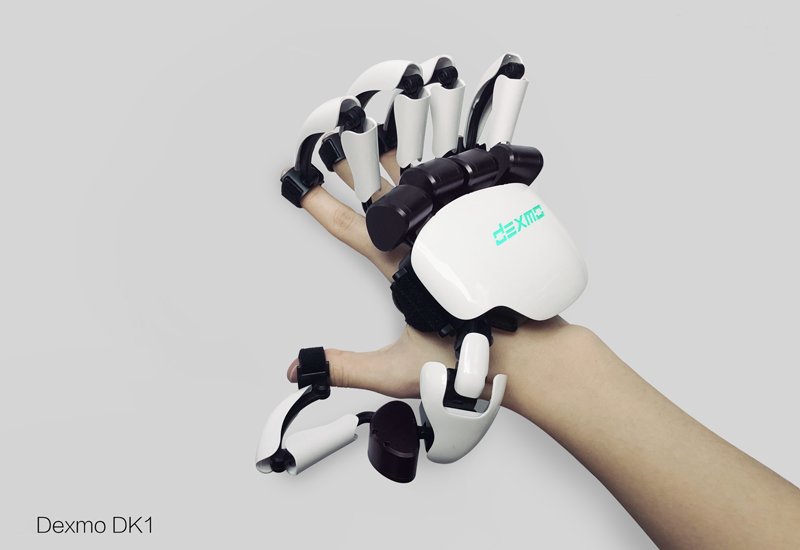
\includegraphics[width=0.7\textwidth]{dexmo}
	\captionsource{Egzoszkielet firmy Dexta Robotics}{\url{https://www.dextarobotics.com/en-us/stories}}
	\label{fig:dexmo}
	\end{figure}	
		\begin{wrapfigure}{l}{0.5\textwidth}
\begin{center}
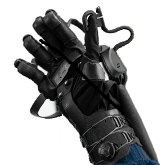
\includegraphics[width=0.46\textwidth]{haptx}
\captionsource{Egzoszkielet firmy HaptX}{\url{https://www.purepc.pl/haptx-glove-pozwoli-na-rejestrowanie-bodzcow-czuciowych-w-vr}}
\label{fig:haptx}
\end{center}
\end{wrapfigure}
	 Kolejnym projektem godnym uwagi jest rękawica HaptX, która pomimo dość dużych rozmiarów, niezbyt zgrabnego wyglądu oraz wagi około 2,5 kg dostarcza wyjątkowe funkcjonalności. Po pierwsze rękawica ta posiada 120 płytek wokół całej dłoni które imitują nacisk przedmiotów w świecie wirtualnym. Płytki te to małe kółka (około 2-3 mm) zgrupowane na płytce po kilka, kilkanaście sztuk w zależności od umiejscowienia na dłoni, w celu lepszej dystrybucji oraz możliwości zarządzania nimi. Rękawica jest na tyle dokładna że można poczuć pojedyncze odnóża chodzącego po dłoni pająka. Firma pracuje również na dodaniem właściwości termicznych do tych płytek co oprócz dotyku pozwoliłoby poczuć temperaturę przedmiotów. W drugiej generacji rękawicy można było poczuć ciepło oraz zimno dzięki zastosowaniu ciepłego i zimnego płynu którymi wyżej wymienione płytki się napełniają. Informację o położeniu naszej dłoni są wyliczane na podstawie dwóch źródeł. Jednym jest śledzenie optyczne naszej dłoni, drugim natomiast położenie naszych palców względem siebie wyliczane dzięki czujnikom magnetycznym które znajdują się na czubkach palców. Rękawica pokazana jest na rysunku~\ref{fig:haptx}~\cite{haptx}.
	 Cyber grasp to rozwiązanie które powstało w 2013 roku, gdy popularność VR znowu zaczęła wzrastać. Jest to egzoszkielet który w pełni kontroluje ruchy naszych palców u dłoni. Jest on nakładany na rękawice które zbiera dane o dłoni. Egzoszkielet jest dość duży i mało przyjazny dla oka, nadrabia to jednak funkcjonalnością oraz solidnym wykonaniem. Zapewnia on pełną swobodę ruchu, do 12 N nacisku oraz możliwość zaprogramowania osobno każdego siłownika oddziałującego na poszczególny palec. Sama rękawica zapewnia osiemnaście sensorów - dwa sensory zgięcia na każdym palcu, cztery sensory odwodzenia pomiędzy palcami, sensor mierzący ruch kciuka, kąt dłoni, a także wygięcie oraz odwodzenie nadgarstka. Istnieje również wersja z czterema dodatkowymi sensorami która zapewnia po jednym dodatkowym sensorze na wszystkie palce poza kciukiem. Oprogramowanie rękawicy wspiera imitację takich odczuć jak pulsowania oraz wibracji dla lepszych doznań ze świata wirtualnego~\cite{cyber}. Ostatnim urządzeniem opisanym w tej sekcji jest rękawica firmy Cynteract. Jest to niemiecka grupa studentów produkująca kontroler w postaci przypominającej egzoszkielet. Nie jest to szkielet w dosłownym tego słowa znaczeniu, a raczej rękawica z zaimplementowanym mechanizmem na wierzchu dłoni, który oddziałuję z małą siłą na palce dłoni. Małe silniki kontrolują napięcie sznurków które wędrują wzdłuż palców aż do samych czubków zapewniając odpowiedni opór. Nie jest to mechanizm który ma na celu powstrzymanie zgięcia dłoni a jedynie stawianie regulowanego oporu. Głównym celem tego produktu jest dotarcie do osób które mają problemy z kontrolowaniem dłoni, dzięki czemu przy użyciu tej techniki mogą dokonywać rehabilitacji w bardziej przyjemny sposób poprzez granie w specjalnie zaprogramowane gry które jednocześnie zbierają dane na temat progresu pacjenta.Rękawica jest uniwersalna dzięki czemu technologia użyta na wierzchniej części może być wymieniania pomiędzy różnymi wersjami tego produktu - oprogramowanie stojąca za działaniem tego mechanizmu jak i rękawicy samej w sobie kryje się w pojemniku umocowanym na nadgarstku. Jest to produkt który nastawiony jest konkretnie na branżę medyczną a jego rozwój wspiera wiele placówek medycznych na terenie Niemiec które już z tego rozwiązania korzystają~\cite{act}. Oprócz wspomnianych projektów istnieje wiele innych rozwiązań implementujących własne rozwiązania problemów kontroli ciała użytkownika. Coraz więcej firm stara się aby ich produktu oprócz wysyłania informacji ze świata rzeczywistego do świata wirtualnego, w celu jak najlepszego odwzorowania użytkownika w tym uniwersum, zapewniało również połączenie w drugą stronę, tak aby ich produkty reagowały na interakcję świata wirtualnego w świecie rzeczywistym, pogłębiając tym samym imersje użytkownika. W tej pracy poruszono jedynie tematykę egzoszkieletów bazujących na kontroli palców, istnieją jednak inne rozwiązania które wykorzystują bardziej skomplikowane systemy, również łączące w sobie wiele rozwiązań z rożnych firm, pozwalające wpływać na poruszanie się ciała użytkownika. W skład tych systemów zazwyczaj wchodzą również rękawice, jednak celem tych produktów nie jest imitacja dotyku poprzez ograniczenie ruchu na której się skupiono w tej sekcji. 